\chapter{Ejercicio 3}
\section{Enunciado}
Un radix tree o PATRICIA es un trie en el cual las cadenas de nodos con un solo hijo
son compactadas y transformadas en un solo nodo. Esto permite mejorar el consumo de
memoria de la estructura en el caso en que hay pocas cadenas definidas o que muchas
cadenas tengan prefijos largos en com'un.

Esta compactaci'on genera entonces las diferencias b'asicas entre los radix trees y los tries:

a) Todos los nodos internos de un radix tree tienen como m'inimo dos hijos (excepto
posiblemente la raiz).

b) Las ramas de un radix tree pueden estar etiquetadas con m'as de un caracter.
Si adem'as el conjunto (o del conjunto de claves del diccionario) es un conjunto libre
de prefijos, sucede que las cadenas (o los valores asociados a las claves) se encuentran
solamente en las hojas. Un conjunto libre de prefijos es aquel en el cual ningun elemento
es prefijo de otro.

Implementar un conjunto de cadenas basado en estas ideas que soporte las siguientes
operaciones:

a) Agregar una cadena al conjunto.

b) Consultar si una cadena pertenece al conjunto.

c) Sacar una cadena del conjunto.

d) Consultar la cantidad de cadenas del conjunto.

Donde las cadenas forman un conjunto libre de prefijos. Las tres primeras operaciones
deben tener complejidad $O( \| s\| )$ \footnote{Posteriormente a la presentaci�n del trabajo, mediante un mail, se inform'o que el orden de la funci�n agregar podia ser $O( \| s \| + t)$ donde t es el largo de la palabra a agregar} donde s es la clave m'as larga ya definida y $\| s \| $ indica la
longitud de s. La 'ultima operaci'on debe tener complejidad de orden constante.

El conjunto de caracteres sobre el que se van a definir las cadenas son las 26 letras min'uscu-
las del ingl'es.

\section{Desarrollo}
\subsection{PATRICIA}
Un \textit{Radix Tree} o \textit{PATRICIA (Practical Algorithm To Retrieve Information Coded In Alphanumeric)} es una estructura de datos 
basada en los \textit{Tries} que suele cumplir el rol de diccionario. Sus claves son cadenas, y su significado es de tipo variado, 
d'andole uso para diferentes prop'ositos. La diferencia entre un PATRICIA y un Trie ya fue mencionada en el enunciado: 
un Trie tiene un nodo por cada caracter de una cadena, en cambio las ramas de un Radix Tree pueden estar etiquetadas con m'as de 
un caracter, y si adem'as el conjunto de claves es libre de prefijos, cada nodo del Radix tendr'a almenos dos hijos.

\subsection{Sobre el dise\~{n}o de la estructura}
Por sus caracter'isticas, el PATRICIA presenta un amplio abanico de posibles implementaciones. Nosotros basicamente pensamos en cuatro formas:
\begin{itemize}
\item Con nodos formados por un arreglo (en este caso de 26 posiciones) que tiene ejes por elementos
\item Con nodos formados por una lista de ejes 
\item Con nodos que contienen una tabla de hash
\item Con nodos que contienen un diccionario sobre AVL
\end{itemize}

Durante este trabajo pr'actico definimos eje como una tupla de puntero a un nodo hijo y una cadena adjunta. Los nodos pueden tener un bit que indica la validez o invalidez del mismo y/o el dato (significado) a guardar. En el caso de este TP, no se piden datos a guardar, por lo que el PATRICIA ser'a conjunto de strings.

Optamos por implementar los nodos con dos variantes de las ya nombradas: nodos formados por un arreglo de 26 posiciones con un bit de existencia y nodos formados por una lista con un bit de existencia. Como luego veremos, ambos dise\~{n}os de estructura cumplir'an las complejidades pedidas. 
El bit de existencia permite que podamos usar el PATRICIA aun en casos donde el conjunto de entrada no este libre de prefijos, 
por ejemplo consideremos la figura \ref{fig:bitExistencia} en este caso si bien la forma del PATRICIA es la misma, 
mediante el bit de existencia podemos diferenciar si la palabra `emi' esta o no definida.

\begin{figure}[H]
\centering
\subfigure[La palabra emi no esta definida]{
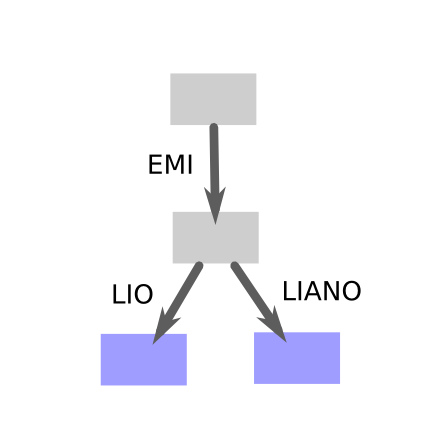
\includegraphics[scale=0.5]{./figuras/ej3/bit_existencia.png} }\hspace{1in} 
\centering
\subfigure[La palabra emi si esta definida]{
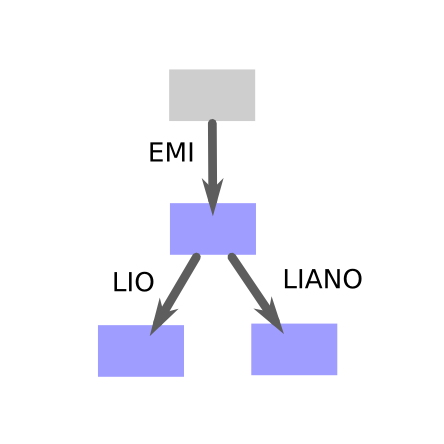
\includegraphics[scale=0.5]{./figuras/ej3/bit_existencia1.png} }
\setcounter{subfigure}{0}
\caption{Utilizaci'on del bit de existencia}
\label{fig:bitExistencia}
\end{figure}

En cuanto al PATRICIA, se decidi'o que el mismo contendr'a nodos y no los definir'a dentro. O sea, separamos la estructura de datos 'arbol PATRICIA de la estructura nodo. Esto es as'i pues de este modo se implementa la modularidad que resulta de gran utilidad para implementar el PATRICIA para los diferentes tipos de nodo elegidos.

\subsection{Sobre el PATRICIA como 'arbol}
El enunciado presenta un invariante para el PATRICIA:
\begin{itemize}
\item Todos los nodos internos de un Radix Tree tienen como m'inimo dos hijos (excepto
posiblemente la raiz).
\item Si adem'as el conjunto (o del conjunto de claves del diccionario) es un conjunto libre
de prefijos, sucede que las cadenas (o los valores asociados a las claves) se encuentran
solamente en las hojas. Un conjunto libre de prefijos es aquel en el cual ningun elemento
es prefijo de otro.
\end{itemize}
Este invariante deber'a conservarse durante todas las funciones.
PATRICIA nos sugiere un 'arbol formado de un conjunto de palabras dispersas en su estructura, como muestra el siguiente gr'afico.

\begin{figure}[H]
\centering
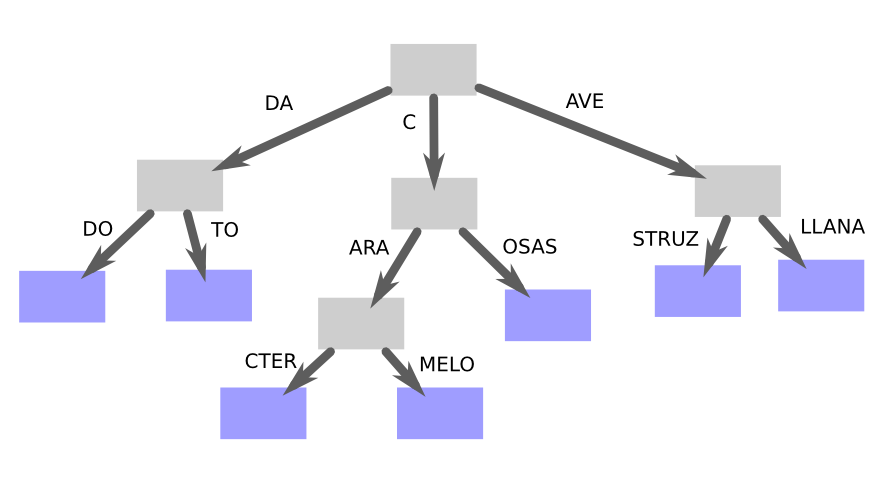
\includegraphics[scale=0.5]{./figuras/ej3/ejemplo_patricia.png}
\caption{Ejemplo de �rbol patricia}
\label{fig:ejemploPatri}
\end{figure}

Los nodos rellenos representan a las claves que pertenecen al conjunto. Este 'arbol se va formando a medida que agregamos y sacamos 
palabras del conjunto. A continuaci'on describiremos cuales fueron las pautas a seguir para armar dichas funciones.

\subsection{Agregando un elemento}
Cuando agregamos un elemento nos enfrentamos ante los siguientes casos:
\begin{itemize}
\item Se puede agregar el elemento sin tener que partir un eje

\begin{figure}[H]
\centering
\subfigure[ ]{
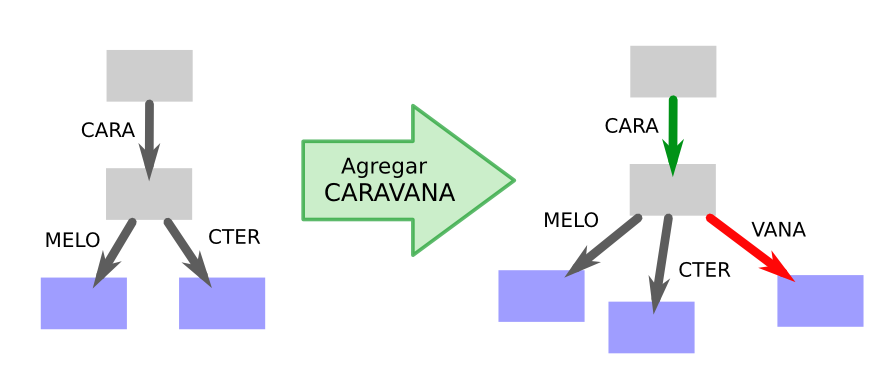
\includegraphics[scale=0.5]{./figuras/ej3/caso1agregar.png} }
\caption{ }
\label{fig:caso1agregar}
\end{figure}

\item Para agregar un elemento, hay que partir un eje y agregar un nodo

\begin{figure}[H]
\centering
\subfigure[ ]{
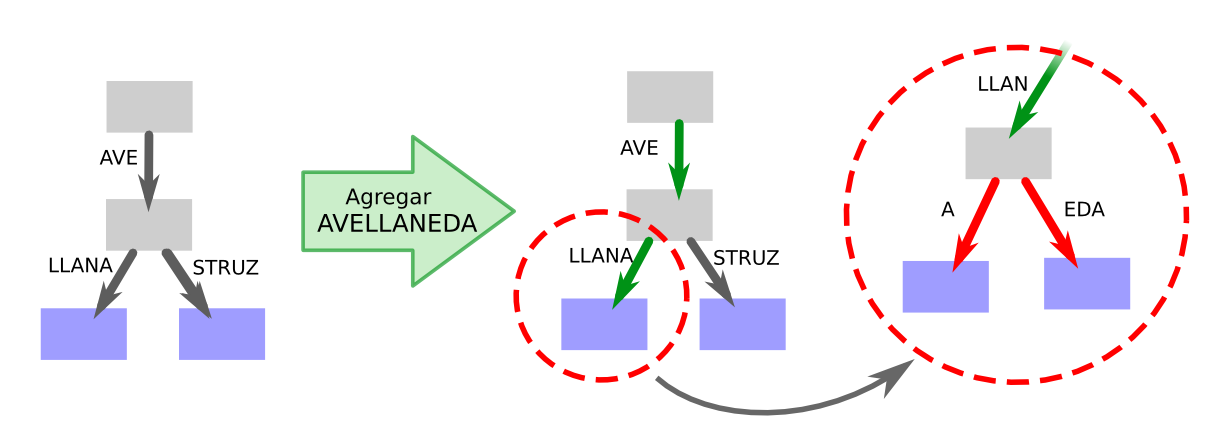
\includegraphics[scale=0.5]{./figuras/ej3/caso2agregar.png} }
\caption{ }
\label{fig:caso2agregar}
\end{figure}

\end{itemize}

Para solucionar estos casos comenzaremos situ'andonos sobre la ra'iz. Luego bajamos por las ramas de la siguiente manera: en cada 
paso mantenemos guardada la palabra formada a partir de la concatenaci'on de las cadenas adjuntas de los ejes por los cuales bajamos, 
y la cadena recortada que resulta de quitarle a la palabra a definir el prefijo en com'un que tiene con cada eje por el cual bajamos.

De esta forma en cada paso buscamos el eje tal que la primer letra de su cadena adjunta coincida con la primer letra de palabra 
recortada. As'i bajaremos por los ejes hasta que encontremos un eje que no sea prefijo, en su totalidad, de la cadena recortada. Este algoritmo no presenta ambiguedades a la hora de buscar el eje por el cual bajar, pues cada nodo tiene un m'aximo de 26 hijos, correspondientes a las 26 
letras del abecedario ingl'es, y no puede tener mas de un eje que su cadena adjunta comience con la misma letra. O sea, no puede 
haber, por ejemplo, ejes con cadenas casa y cosa en el mismo nodo.

Una vez que bajamos por las ramas lo m'aximo posible, si la palabra formada es prefijo de la palabra a agregar, quiere decir que 
caimos en el primer caso. Este caso es simple y solo resta agregar el nodo y el eje correspondiente, con la palabra sin prefijo, 
como se muestra en la figura \ref{fig:caso1agregar}.

Si la palabra formada no es prefijo de la clave a definir, este es el segundo caso, pues esto querr'a decir que el 'ultimo eje tiene letras que son parte de la clave y otras que no lo son. En este las partes involucradas ser'an: el padre del nodo actual (lo llamaremos $p$), el 'ultimo eje por el cual bajamos, que apunta al nodo actual (llamemoslo $j$), y el nodo actual(lo llamaremos $n$). Entonces haremos lo siguiente: "`partimos"' $j$ en las partes $j_1$ y $j_2$. La primera se corresponde con la 'ultima parte del prefijo de s, y la segunda son las letras que no coincidieron con s. Creamos un nuevo padre (desde ahora $p'$), de manera que $j_1$ quedar'a apuntando desde $p$ a $p'$, y $j_2$ apunta desde $p'$ a $n$. Finalmente, para reestablecer el invariante, agregamos un nuevo nodo y un nuevo eje, apuntando desde $p'$ al nuevo nodo, que tenga adjunto la parte restante de la clave (ver figura \ref{fig:caso2agregar}).

Excediendo el l'imite del enunciado, nuestro algoritmo agregar podr'a tener en cuenta conjuntos de entrada que no sean libre de 
prefijos. Esto nos agregar'a dos casos m'as: 
\begin{itemize}
\item Para agregar un elemento hay que simplemente setear el bit de existe

\begin{figure}[H]
\centering
\subfigure[ ]{
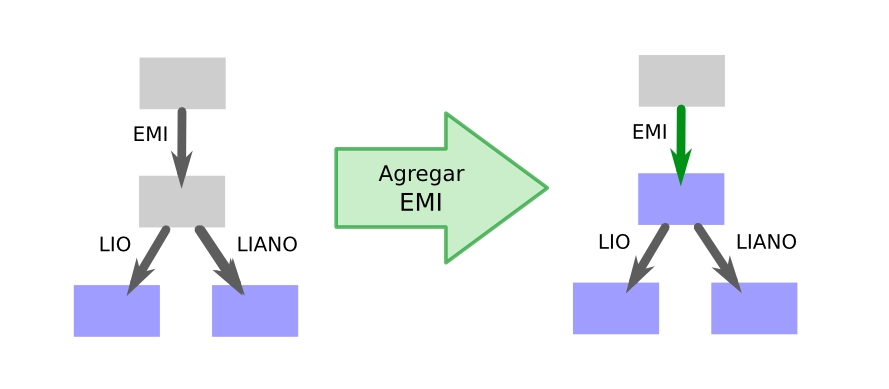
\includegraphics[scale=0.5]{./figuras/ej3/caso3agregar.png} }
\caption{ }
\label{fig:caso3agregar}
\end{figure}

\item Para agregar un elemento hay que partir un eje y setear el bit de existe
\end{itemize}
\begin{figure}[H]
\centering
\subfigure[ ]{
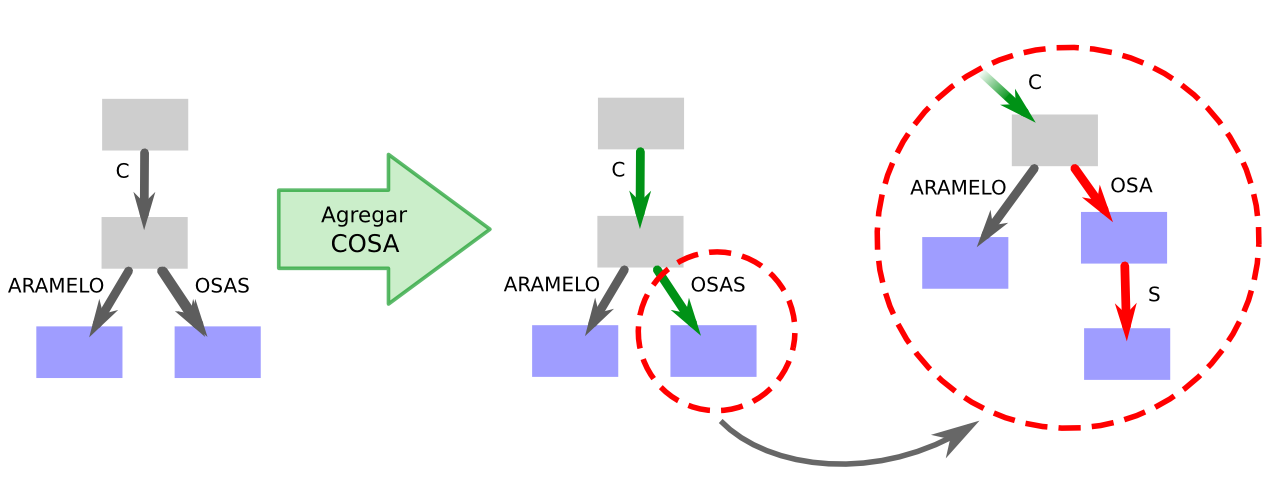
\includegraphics[scale=0.5]{./figuras/ej3/caso4agregar.png} }
\caption{ }
\label{fig:caso4agregar}
\end{figure}

Estos dos nuevos casos en realidad podemos resolverlos como derivados de los dos anteriores. Si al bajar por las ramas, la 
palabra formada es prefijo de la clave, y la clave es prefijo de la palabra formada, o sea que la clave y la palabra formada son iguales, caemos en el primer caso. En este caso simplemente se setea el bit de existe al nodo en el cual caimos, como lo muestra la figura \ref{fig:caso3agregar}.

Si al bajar por las ramas, la clave es prefijo de la palabra formada y la palabra formada es m'as larga que la clave, caemos en el 
segundo caso. Este problema se resuelve partiendo el eje y creando un nuevo nodo en medio del eje a partir. Ahora la primer parte del eje partido apuntar'a al nuevo nodo, y la parte restante apuntar'a desde el nuevo nodo hacia el nodo en el cual caimos al bajar, como lo muestra la figura \ref{fig:caso4agregar}.
Claramente los dos primeros casos correspondientes al enunciado son excluyentes con estos dos 'ultimos casos, pues los primeros agregan solo nodos hojas, los segundos agregan solo nodos internos. Esto me asegura que el producto pedido no ser'a cambiado.

\subsection{Eliminando un elemento}
Cuando eliminamos un elemento nos enfrentamos ante los siguientes casos:
\begin{itemize}
\item Para sacar un elemento hay que eliminar un nodo y un eje
\begin{figure}[H]
\centering
\subfigure[ ]{
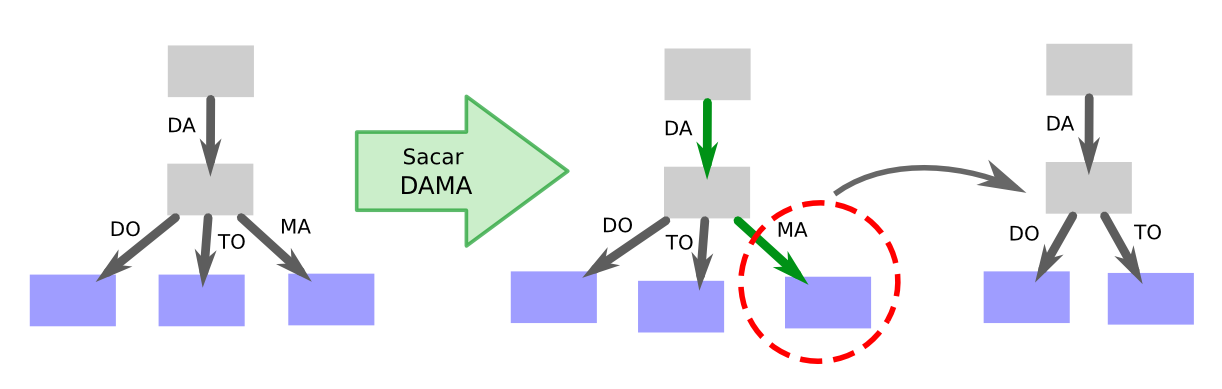
\includegraphics[scale=0.5]{./figuras/ej3/caso1sacar.png} }
\caption{ }
\label{fig:caso1sacar}
\end{figure}

\item Para sacar un elemento hay que eliminar el nodo con su eje, borrar el padre y concatenar dos ejes
\end{itemize}
\begin{figure}[H]
\centering
\subfigure[ ]{
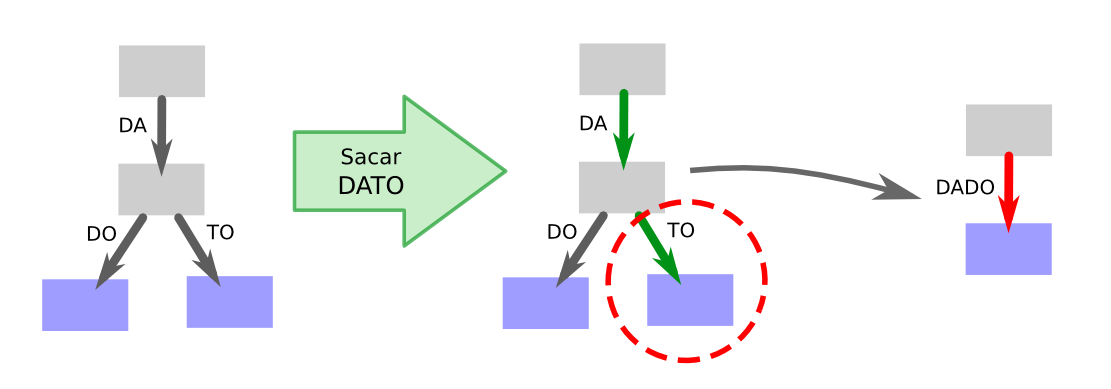
\includegraphics[scale=0.5]{./figuras/ej3/caso2sacar.png} }
\caption{ }
\label{fig:caso2sacar}
\end{figure}
Para solucionar estos casos comenzamos situ'andonos sobre la ra'iz, y bajando, al igual que agregar. El valor asociado a la clave se encuentra en la hoja, pues el Radix es libre de prefijos, por lo que solo eliminaremos hojas.
Al borrar una hoja, debemos verificar cuantos hermanos ten'ia. Si ten'ia m'as de un hermano, caeremos en el primer caso, 
el cual se resuelve simplemente eliminando la hoja y su eje, como lo muestra el gr'afico \ref{fig:caso1sacar}.
Si, por el contrario, ten'ia solo un hermano, al borrar este nodo al padre le restar'a un solo hijo. Para reestablecer el invariante, como la rama hasta el nodo padre no conforma una clave definida, podemos unir el padre con su 'unico hijo. Lo hacemos simplemente borrando el nodo hijo y concatenando el eje que apunta del nodo abuelo al nodo padre con el eje que apunte del nodo padre al
 nodo hijo, como lo muestra el grafico \ref{fig:caso2sacar}.

Excediendo el l'imite del enunciado, nuestro algoritmo sacar podr'a tener en cuenta conjuntos de entrada que no sean libre de 
prefijos. Esto nos agregar'a dos casos m'as: 
\begin{itemize}
\item Para sacar un elemento hay que setear FALSE el bit de existe
\begin{figure}[H]
\centering
\subfigure[ ]{
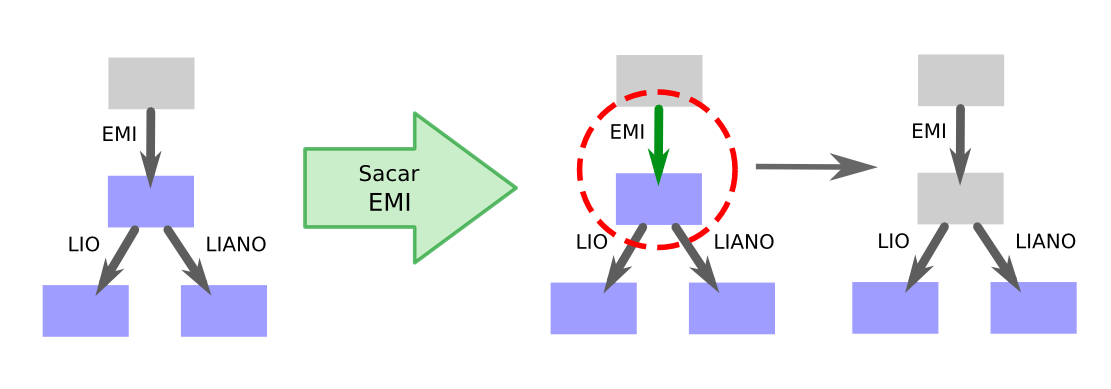
\includegraphics[scale=0.5]{./figuras/ej3/caso3sacar.png} }
\caption{ }
\label{fig:caso3sacar}
\end{figure}

\item Para sacar un elemento hay que concatenar dos ejes y borrar un nodo

\begin{figure}[H]
\centering
\subfigure[ ]{
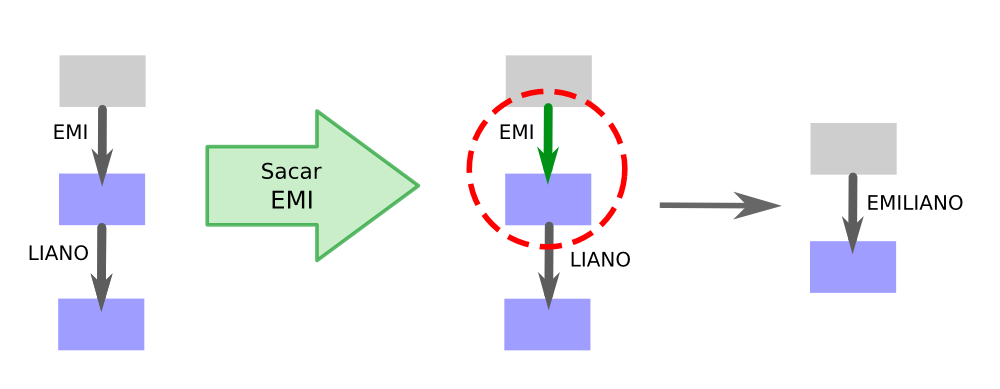
\includegraphics[scale=0.5]{./figuras/ej3/caso4sacar.png} }
\caption{ }
\label{fig:caso4sacar}
\end{figure}

\end{itemize}
Estos dos nuevos casos son consecuencia directa de los casos de entrada que no esta libre de prefijos de agregar. 
Luego de bajar por las ramas del 'arbol verificamos que la palabra armada es igual a la clave y el nodo existe. De esta forma nos
 aseguramos que la clave a borrar haya sido definida. Si el nodo a borrar es un nodo interno (no es una hoja), caemos en alguno
 de estos dos casos. Si el nodo a borrar tiene m'as de un hijo, caemos en el primer caso. Este se soluciona seteando el bit de 
 existencia del nodo a falso, como muestra la figura \ref{fig:caso3sacar}. Si el nodo a borrar tiene solo un hijo, este es
 el segundo caso. Se resuelve borrando el nodo padre y concatenando el eje que apuntaba del nodo padre al nodo actual, y el eje
 del nodo actual al nodo siguiente, como lo muestra la figura \ref{fig:caso4sacar}.
 
Claramente estos dos casos son excluyentes con los dos primeros correspondientes al enunciado, pues en ellos se borran solo hojas, mientras que estos ultimos se borran nodos internos.

\subsection{Pertenencia de una cadena al conjunto}
La idea es bajar por los ejes que son prefijos de s, hasta que o bien completamos s o bien no tenemos ejes que sean prefijo de s. Si completamos s, revisamos que el nodo exista y si esa asi se devuelve verdadero; en otro caso devolvemos false.

\subsection{Cardinal}
Dado que se nos ped'ia devolver el cardinal en orden constante, no nos qued'o otra alternativa que tenerlo calculado cuando se llame a la funci'on. Por eso, tenemos el valor calculado, increment'andolo y decrement'andolo cuando se agrega o saca una palabra, respectivamente.

\section{Cuestiones de implementaci'on de los nodos y del PATRICIA}
Con respecto a las listas (para los nodos que las usan) usamos las provistas por la Standard Template Library (STL). Un nodo guarda la cantidad de hijos que tiene y si 'el existe. Si bien aislando el nodo como estructura independiente, el booleano `` existe' puede carecer de sentido, lo adquiere al implementar el PATRICIA, ya que sin ella no podriamos diferenciar los elementos definidos de los no definidos. La cantidad de hijos es 'util para saber cuantos hijos contiene un nodo implementado sobre arreglos.

La implementaci'on de nodos sobre arreglos cuenta con un arreglo de apuntadores a eje, an'alogamente la implementaci'on con listas cuenta con una lista con apuntadores a ejes. Un eje, es una cadena asociada y un puntero a otro nodos.

Cada nodo es capaz de agregar nodos hijos mediante un eje con una cadena adjunta, siempre y cuando no tenga hijos cuya cadena asociada a su eje comience con la misma letra. El nodo hijo lo puede crear o recibirlo como un parametro.
Asimismo, un nodo es capaz de sacar un eje que lo une a alguno de sus hijos, sin embargo no borra a dicho hijo, esto ser'a tarea del PATRICIA.

%TODO: creo q alcanza con lo q dije antes

%A continuaci'on explicaremos detalladamente cada funci'on referente a los nodos:
%\begin{itemize}
%\item constructor: inicializa el booleano existe a FALSE. En caso de nodo sobre arreglo, inicializa adem'as cantElem a 0 (cero) y todo el arreglo a NULL.
%\item agregar: toma por par'ametro una referencia constante a cadena y un opcional apuntador a nodo. Adhiere un nuevo nodo al conjunto de hijos del nodo en cuesti'on. Lo hace asign'andole un eje que tiene un puntero al nuevo nodo y una cadena adjunta. Si el nodo es pasado por par'ametro, el eje apuntar'a hacia ese nodo. Caso contrario se crear'a un nuevo nodo sin nodos hijos, con el bit existe en TRUE, y el eje apuntar'a hacia el nuevo nodo. Esto es as'i a causa de efectos pr'acticos a la hora de implementar el PATRICIA. Para el caso de los nodos sobre arreglos, a la i-esima letra del abecedario ingl'es le corresponde la i-esima posici'on del arreglo. En caso de los nodos sobre listas, los ejes son agregados en orden ascendiente por cadena.
%
%\item sacar: toma por par'ametro una referencia constante a cadena. Borra el eje adjunto a la cadena pasada por par'ametro. No borrar'a el nodo apuntado por el eje borrado. Esto, en cambio, ser'a tarea del PATRICIA. Para el caso de los nodos sobre arreglos, borrar el eje es trivial si indexamos el arreglo  sobre la primer letra del par'ametro. En cambio, para los nodos sobre listas, se deber'a iterar sobre la lista hasta encontrar el eje a borrar.
%
%\item pertenece: toma por par'ametro una referencia constante a cadena. Verifica si existe un eje adjunto a la cadena pasada por par'ametro. Para los nodos sobre arreglos, indexamos el arreglo sobre la primer letra del par'ametro y verificamos la igualdad. Para los nodos sobre listas, iteramos sobre la lista hasta encontrar la cadena buscada. Para ambos casos, si no se encuentra un eje adjunto a la cadena, se devuelve NULL.
%
%\item ejeQueEmpiezaCon(cadena): toma por par'ametro una referencia constante a cadena. Requiere que la cadena sea de longitud 1 (uno). Caso contrario devolver'a NULL. Devuelve un puntero a eje que tiene por primer letra el parametro. Para nodo sobre arreglos, simplemente se indexa sobre la letra del par'ametro. Para nodo sobre listas, se itera sobre la lista de ejes, hasta encontrar una coincidencia entre la primer letra de la cadena adjunta al eje iterado con el par'ametro. Si no existe tal eje, se devuelve NULL.
%
%\item iesimoEje(entero): toma por par'ametro un entero sin signo $n$. Devuelve un apuntador a eje. Para nodo sobre arreglos, se indexa el arreglo sobre el entero pasado par'ametro. Para nodo sobre listas, se itera sobre la lista de ejes, hasta iterar $n$ veces. Si no existe tal eje, se devuelve NULL.
%
%\item primerEje: no toma par'ametros. Devuelve un apuntador al primer eje encontrado. Para nodo sobre arreglos, se busca de 0 a 26 un eje definido. Para nodo sobre listas, se devuelve el primer elemento de la lista.
%
%\item cantHijos: no toma par'ametros. Devuelve el cardinal del nodo, entendi'endose por cardinal la cantidad de hijos que tiene. En realidad esta funci'on no hace mas que devolver el valor de la variable cantElem.
%
%\item esHoja: no toma par'ametros. Devuelve TRUE o FALSE indicando si el nodo no tiene ningun nodo hijo o tiene alguno, respectivamente. Simplemente se compara cantElem con 0.
%
%\item destructor: para nodo sobre arreglo, recorre el arreglo eliminando eje por eje (NO borra los nodos hijo). En caso de nodo sobre lista, no hace absolutamente nada.
%\end{itemize}

Definimos la clase PATRICIA que es `` amiga '' de la clase nodo. Necesita ser amigo para tener acceso a la creaci'on de ejes y uso de los m'etodos privados. El PATRICIA est'a compuesto entonces por un nodo llamado ra'iz y por la cantidad de palabras definidas. Esta 'ultima variable la necesitamos para poder cumplir con el orden pedido para la funci'on cardinal.

A la hora de agregar, optamos por copiar la cadena s de entrada, ya que nos pareci'o que era mas prolijo, pues la otra forma que no requer'ia copiar la cadena era usando una referencia de entrada, ir rompi'endola y guard'andola en el eje correspondiente; sin embargo es probable que un potencial usuario de este conjunto no desee que si le pasa una palabra se le destruya. Si bien nos desmejor'o un poco el orden (como se ver'a m'as adelante el orden es O($long_s + long_{max}$) creemos que hace que el conjunto sea m'as ameno de usar.

%TODO: y si mejor nos hacemos los pelotudos?
Para el manejo de las cadenas, usamos string de la STL. Para las mismas necesitamos que la concatenaci'on de una cadena s a una cadena t sea O(s), que comparar dos cadenas s y t se pueda hacer en O(min($long_s$,$long_t$)). Si bien no pudimos encontrar los ordenes en los que la STL provee estas operaciones, son ordenes faciles de cumplir, por lo que podemos suponer que valen.

%\begin{itemize}
%\item constructor: inicializa cantElem a 0 (cero) y la raiz, sete'andole TRUE a su valor existe.
%
%\item destructor: hace un recorrido postorder sobre el 'arbol: primero recorre la lista de hijos, llamando recursivamente, y luego borra el nodo actual.
%
%\item agregar: toma por par'ametro una referencia constante a cadena. Se baja por las ramas con el m'etodo bajar. Se verifica si la palabra armada es igual a la cadena y si el nodo existe. Si esto se cumple, terminar'a, pues quiere decir que la palabra ya estaba definida, sino sigue su ejecuci'on. A partir de este paso, sabemos que hay un elemento que ser'a agregado, pues es un elemento no existente en el conjunto. Luego se toma la cadena pasada por par'ametro y la palabra armada, y se les quita el prefijo. Esto lo hacemos pues as'i podemos ver si debemos partir el eje o no, ya que si la palabra armada, que es la concatenaci'on de todos los ejes por los que baj'e, no es prefijo de la cadena, quiere decir que el 'ultimo eje no coincid'ia totalmente con la parte de la cadena sin prefijo. Verificamos entonces si la palabra armada es vac'ia luego de sacarle el prefijo, si no lo es, partimos el eje y creamos un nuevo padre para este nodo. Si era vacia, no hacemos nada. Luego dependiendo si se partio el eje o no, colgamos el nuevo nodo del nuevo padre o del nodo en el que quedamos luego de bajar, y a ese eje le adjuntamos la parte sin prefijo de la cadena, con el m'etodo agregar de nodo. Finalmente se incrementa la variable cantElem, sin importar en qu'e caso entr'o, pues antes hab'iamos comprobado si la cadena a agregar no est'a definida en el conjunto.
%
%\item sacar: toma por par'ametro una referencia constante a cadena. Se baja por las ramas con el m'etodo bajar. Se verifica si se logr'o encontrar la cadena comparandola en relaci'on de igualdad con la palabra armada, y si el nodo existe. Si esto se cumple, el algoritmo sigue su ejecuci'on, sino termina. Nuevamente decimos que a partir de este paso, sabemos que hay un elemento que ser'a eliminado. Para este m'etodo resulta necesario el retorno de bajar, el eje anterior al eje actual (el que va del abuelo al padre del nodo actual), pues este nos permite resolver casos de uni'on de ejes cuando el padre del actual tiene dos hijos o menos. Empezamos por resolver los casos que el enunciado nos da: aquellos que borramos una hoja. Si el actual es hoja, lo borramos, junto con su eje, y verificamos lo siguiente: si exist'ia un nodo anterior (no se est'a borrando ning'un elemento que esta colgado de la raiz) y el anterior no existe y, luego de borrar la hoja, tiene 1 hijo, entonces tenemos que unir los ejes anterior y el eje que va del padre al 'unico hermano del nodo borrado. Los casos restantes son aquellos que se debe borrar un nodo interno. Estos se contemplan entre todo el conjunto de casos que son disjuntos con el anterior (aquellos en los que se borran hojas). Se comienza preguntando si el nodo actual tiene un unico hijo, pues debemos evitar podar toda una rama del 'arbol incorrectamente. En este caso, se concatenan los ejes del padre del actual al actual, y del actual al hijo del actual. Luego se procede a borrar el actual. Si el actual tenia m'as de un hijo, se setea el bit existe a FALSE. Finalmente se decrementa la variable cantElem en uno. Es importante notar que la variable decrementa sin importar en qu'e caso entr'o, pues antes hab'iamos comprobado si la cadena a borrar est'a definida en el conjunto.
%
%\item pertenece: toma por par'ametro una referencia constante a cadena. Devuelve un booleano. Se procede bajando por el 'arbol con el m'etodo bajar, y se verifica si se logr'o encontrar la cadena comparandola en relaci'on de igualdad con la palabra armada, y si actual existe.
%
%\item cardinal: no toma par'ametros. Devuelve un entero positivo. Esta funci'on devuelve el valor de cantElem.
%
%\item bajar: toma por par'ametro una referencia a puntero a nodo, una referencia a puntero a eje, una referencia constante de cadena, y una referencia a cadena. Devuelve un puntero a eje. El primer par'ametro corresponde al nodo actual, y funciona como variable para devolver resultados. Al algoritmo no le interesa lo que le manden en esa variable, pues al entrar define actual como raiz. An'alogamente, el segundo par'ametro funciona tambi'en como variable de retorno del eje actual (el que apunta al nodo actual) y el algoritmo asigna su valor al entrar a la funci'on. El tercer par'ametro es la cadena que se le pasa por par'ametro a agregar y a bajar. El cuarto par'ametro es la palabra armada, que es la concatenacion de todas las cadenas adjuntas a los ejes por los cuales bajaremos. A este par'ametro tambi'en se le asigna un valor, que es la cadena vac'ia, apenas se llama la funci'on. Este m'etodo tiene como fin ser reciclable: puede ser usado para bajar por el 'arbol, sin importar el caso para el cual se lo quiere usar, sea agregar, sacar o verificar pertenencia.
%Bajar define cuatro variables auxiliares: puedeBajar (bool), recortada (string), aux (puntero a eje) y ejeAnterior (puntero a eje). La primera define si el algoritmo puede seguir bajando o no por las ramas del 'arbol, la segunda sirve para guardar la parte que falta por recorrer del tercer argumento, la tercera sirve para mirar a los ejes antes de bajar, y la cuarta guarda el valor de ejeActual (segundo par'ametro) antes de ser cambiado. El m'etodo comienza llamando a actual.ejeQueEmpiezaCon d'andole la primer letra de recortada (que al principio coincide con la primer letra del tercer par'ametro). Si existe tal eje, se asigna TRUE a puedeBajar. Sino, el algoritmo finaliza. Si es cierto que se puede bajar, se procede a hacerlo actualizando los valores de eje anterior, eje actual, nodo actual, la palabra armada, la palabra recortada y puedoBajar. A puedoBajar se le asigna TRUE si el eje actual es prefijo (completo) de recortada. Sino se le asigna falso. Este procedimiento se ejecuta hasta que puedoBajar sea falso, sea porque lleg'o a una hoja o porque el eje que contiene eje actual no es totalmente prefijo de recortada.
%
%\item quitarPrefijoEnComun: toma por par'ametro una referencia a cadena y una referencia constante a cadena. Recorre letra por letra de los par'ametros, hasta que alguno de los dos llegue al final, y guarda un contador de cu'antas letras recorri'o. Al finalizar, le borra al primer par'ametro desde el principio de la cadena hasta contador. La funci'on devuelve TRUE si la longitud del segundo par'ametro es igual al valor de contador, o sea devuelve true si el segundo par'ametro es prefijo del primero. Caso contrario, devuelve FALSE.
%\end{itemize}

\section{Pseudoc'odigo}
\begin{algorithm}
\caption{baja por las ramas segun una cadena s, ademas va armando la palabra que se forma durante el recorrido }
\begin{algorithmic}[1]
\PARAMS{una cadena s y otra cadena, cadenaArmada que se va a modificar}
\STATE cadenaArmada \textcolor{orange}{$\leftarrow$}  $""$
\STATE ejeAnterior \textcolor{orange}{$\leftarrow$}  \textcolor{orange}{$\bot$}
\STATE ejeActual\textcolor{orange}{$\leftarrow$}  \textcolor{orange}{$\bot$}
\STATE nodoActual \textcolor{orange}{$\leftarrow$} raiz
\STATE eje \textcolor{orange}{$\leftarrow$} eje de nodo actual que comienza con la primer letra de s
\STATE puedoBajar \textcolor{orange}{$\leftarrow$} (existe dicho eje);
\WHILE{ exista el eje \textcolor{orange}{$\wedge$} puedoBajar }
	\STATE guardamos en eje anterior el ejeActual
	\STATE guardamos en ejeActual el eje que estamos mirando ahora 
	\STATE nodoActual \textcolor{orange}{$\leftarrow$} nodo apuntado por el eje
	\STATE palabraArmada \textcolor{orange}{$\leftarrow$} palabraArmada \textcolor{orange}{++} cadena del eje
	\STATE sacar a s la parte del eje que le es prefijo
	\STATE puedoBajar \textcolor{orange}{$\leftarrow$} el eje entero era prefijo de s
	\STATE eje \textcolor{orange}{$\leftarrow$} eje del nodo actual que empieza con la primer letra de s
\ENDWHILE
\RETURN ejeAnterior
\end{algorithmic}
\end{algorithm}	

\begin{algorithm}
\caption{agrega una palabra s al conjunto}
\begin{algorithmic}[1]
\PARAMS{ la palabra s a agregar}
\STATE bajar por las ramas hasta no encontrar mas prefijo en el trie
\STATE palabraArmada \textcolor{orange}{$\leftarrow$} palabra armada durante el recorrido
\STATE acutal \textcolor{orange}{$\leftarrow$} nodo hasta donde baje
\STATE ejeActual \textcolor{orange}{$\leftarrow$} eje que apunta al nodo actual
\IF{si la palabra ya esta definida}
	\STATE no hacer nada
\ELSE
	\STATE elminar prefijos comunes de s y de palabraArmada
\IF{palabrArmada $\neq$ $""$} %\COMMENT{}
		\STATE \COMMENT{hay que partir un nodo} 
		\STATE existia \textcolor{orange}{$\leftarrow$} nodoActual.existe
		\STATE ejeActual.cadena \textcolor{orange}{$\leftarrow$} Ejactual.cadena \textcolor{orange}{-} palabraArmada  \COMMENT{dejar en el eje actual la parte que concidia con s}
		\STATE padreActual \textcolor{orange}{$\leftarrow$} nuevoNodo 
		\STATE crear eje (j) entre padreActual y nodoActual
		\STATE cadena de j \textcolor{orange}{$\leftarrow$} palabraArmada
		\STATE apuntar ejeActual a nuevoPadre 
		\IF{existia}
			\STATE poner que existe el nodoActual
		\ELSE
			\STATE poner que no existe el nodoActual
		\ENDIF
\ENDIF
\ENDIF
	\IF{ si s $\neq$ $""$}
		\STATE agregar un eje con s al nodo actual
		\STATE poner un nodo al final de ese eje, con el existe en true
	\ELSE
		\STATE setear el existe del nodo actual en true
	\ENDIF
\STATE palabras definidas \textcolor{orange}{++}
\end{algorithmic}
\end{algorithm}

\begin{algorithm}
\caption{determina si una palabras esta en el conjunto}
\begin{algorithmic}[1]
\PARAMS{ la palabra s a buscar}
			\STATE bajar por las ramas hasta que no quede mas prefijo
			\STATE palabraArmada \textcolor{orange}{$\leftarrow$} palabra armada durante el recorrido
			\RETURN palabraArmada \textcolor{orange}{==} s \textcolor{orange}{$\wedge$} el nodo existe
\end{algorithmic}
\end{algorithm}		






\begin{algorithm}[H]
\caption{saca una palabra s del conjunto}
\begin{algorithmic}[1]
\PARAMS{ la palabra s a sacar}
\REQUIRE{que la palabra a sacar halla sido agregada}
\STATE bajar por las ramas hasta no encontrar mas prefijo
\STATE ejeAnterior \textcolor{orange}{$\leftarrow$} ultimo eje que pase
\STATE actual \textcolor{orange}{$\leftarrow$} nodo en el que quede parado
	\IF{ el nodo actual es una hoja}
		\STATE elminar nodo y eje
		\IF{el padre de la hoja ahora solo tiene un hijo, y el no esta definido} \STATE \COMMENT{si el nodo esta definido, es porque el conjunto no era libre de prefijos}
		\STATE agregar al eje del padre, la cadena del eje del hijo
		\STATE linkear al padre con los hijos de su hijo
		\STATE borrar al hijo
		\STATE setear al padre como definido
		\ENDIF
	\ELSE
		\IF{el nodo a borrar tiene solo un hijo}
		\STATE \COMMENT{este caso no puede ocurrir en un conjunto libre de prefijos}
		\STATE combinar las cadenas del eje desde el padre de actual a actual y el eje desde actual a su hijo 
		\STATE borrar actual
		\ELSE
				\STATE \COMMENT{tiene mas de un hijo}
				\STATE setear actual como no definido
		\ENDIF
	\ENDIF
	\STATE una palabra definida menos
\end{algorithmic}
\end{algorithm}		

%TODO: que alguien me revise, por el amor de Dios!!!!!!!!!!!!!!!!!
\section{C�lculo de complejidad}
Para realizar el an'alisis de la complejidad vamos a considerar el modelo uniforme ya que las principales operaciones se realizan a nivel de caracteres, por lo cual podemos considerar que tienen un costo acotado. Ahora bien, con respecto al tama�o de la entrada, en este caso consideramos que es la cantidad de caracteres que componen a la cadena sobre la que se va a operar, ya sea para agregarla, borrarla o saber si est'a definida. Llamo $s$ a la cadena de entrada, y $long_s$ al largo (cantidad de caracteres) de la misma y $long_{max}$ a la longitud de la cadena m'as larga ya agregada.

A continuaci'on analizaremos las cuatro funciones que deb'iamos implementar, para determinar el orden de complejidad logrado en cada una.
\subsection{Bajar}
Primero inicializamos algunas variables que son punteros. Incializamos tambi'en eje, para hacerlo, buscamos el eje que sale del nodo y comienza con la misma letra que s. En los arreglos lo hacemos en O(1).
 
Por otro lado, con las listas ocurre lo mismo, ya que a lo sumo hay 26 caracteres, es decir 26 ejes de salida para el nodo. Por lo tanto, como es una cantidad acotada por una constante, recorrer esa lista tambi'en es O(1). 

Luego viene un ciclo (l'inea 7), que itera mientras el eje exista y pueda bajar. Poder bajar, salvo en la primer iteraci'on en la cual tiene el mismo significado que existe el eje, significa que el eje entero sea prefijo de s. Ambas condiciones se pueden dar como m'aximo $long_{max}$ veces, ya que no puede haber m'as ejes con prefijo en s que la cantidad de ejes para guardar a la palabra m'as larga, que tiene dicha longitud.

Dentro del ciclo, lo que hacemos es asignar ciertos punteros en O(1), buscar el eje por donde seguir, tambi�n en O(1), concatenar a la cadenaActual la cadena del eje que acabamos de pasar y sacar de s el prefijo del eje. Hay que notar que si en una iteracion concatenamos a palabraArmada una cadena de largo k, el m'aximo n'umero de ejes es $long_{max}$ - k, ya que como mucho podemos tener $long_{max}$ ejes de un caracter.

Entonces si el ciclo hace n iteraciones, y tenemos que en la cantidad de caracteres del i-'esimo eje que visitamos es $k_i$, vale que:
$$\sum_{i=1}^{n}{k_i} \leq long_{max}$$

Es por esta raz'on que la complejidad del algoritmo es O($long_{max}$).
  
\subsection{Agregar}
Lo primero que hacemos es bajar por las ramas mientras encontremos prefijo para s, como vimos en el apartado anterior, el costo de esto es O($long_{max}$).

Si la palabra ya estaba en el conjunto(l'inea 5), no hacemos nada y terminamos. El costo fue en total $O(long_{max})$.

Si en cambio la palabra no estaba, lo pr'oximo que hacemos es eliminar los prefijos comunes entre s y la palabra armada durante el descenso (l'inea 8) , nuevamente para hacer esto, recorremos a lo sumo $long_{max}$ caracteres, ya que lal cadenas de los ejes de una rama no pueden tener mas caracteres que $long_{max}$.

Si hay que partir el nodo, lo que se hace es partir la cadena del 'ultimo eje visitado en la parte que es igual a s y la parte que difiere (l'inea 12). Para partir esta cadena, se recorren tantos caracteres como prefijo de s haya en el PATRICIA, y esta cantidad est'a acotada por $long_{max}$ caracteres.

Una vez que partimos esta cadena creamos un eje nuevo, que se hace en O($long_{max}$), porque si armamos un eje nuevo hay que copiar la parte de la cadena del eje, que no era prefijo en s(l�nea 14). Tambi'en creamos un nuevo nodo, que se hace en O(1).

Luego de esto, linkeamos los nodos mediante el eje antes creado, y seteamos el valor de existencia del nodo. Estas acciones se hacen en O(1), lo primero es setear un puntero y lo segundo es asignar un bool.

Despu'es de esto, si hay que agregar un nuevo eje para s, se hace, pero esta vez el costo es O($long_s$), puesto que s podria ser en principio mayor que la palabra de longitud m'axima entre las definidas(l�nea 25). Se crea un nuevo nodo y se linkea con el nodo hasta donde hab'ia bajado en O(1).

Si no hab'ia que partir nodo, ni agregar un nodo nuevo, solo se setea el bit de existe en el ultimo nodo que visite (l'inea 28) .

Por 'ultimo si la palabra no estaba ya en el conjunto, incrementamos en uno el cardinal del conjunto.

Luego tenemos una cantidad acotada de operaciones de costo O($long_s$) y O($long_{max}$). Por lo tanto la complejidad del algoritmo es O($long_s$+$long_{max}$), es decir O(max($long_s$+$long_{max}$))

\subsection{Sacar}

Primero bajamos mientras en los ejes encontremos prefijo de s. Esto se hace en $O(long_{max})$. Notemos que como para poder sacar una palabra, pedimos como precondici'on que s haya sido agregada, sabemos que $long_s$ $\leq$ $long_{max}$. Entonces en verdad esta bajada tiene costo $O(long_s)$.
 
Si el nodo a borrar es una hoja, eliminamos el nodo y al eje correspondiente(l�nea 5). Borrar el eje, tiene $O(long_s)$ porque dicho eje, era subcadena de s.  

Una vez hecho esto, podr'ia ser necesario, si el padre tiene ahora solo un hijo, combinar el string del eje que llega al padre con el de su hijo. Esto se hace en O($long_{max}$) ya que no sabemos a priori que tan largo puede ser la cadena del eje del ``hermano'' de s (l�neas 8 a 11).

Si no era una hoja y tiene solo un hijo lo que hacemos es borrar el nodo, y combinar los ejes de 'el con su padre y de 'el con su 'unico hijo. Nuevamente el costo de esto es O($long_{max}$) (l�neas 16 y 17).

Si no era hoja y no tenia solo un hijo, lo que hacemos es setear su flag de existe en false, que se hace en O(1). 

Lo ultimo que hacemos es decrementar en uno el cardinal del conjunto en O(1).

Luego el orden de esta operacion es  O($long_s$+$long_{max}$), pero como $long_s \leq long_{max}$, O($long_s$+$long_{max}$) es O(max($long_s$,$long_{max}$)), que es O($long_{max}$)

\subsection{Pertenece}
Al igual que con las dos operaciones anteriores, lo que hacemos es bajar mientras encontremos en los ejes, prefijos de s. Esto, como dijimos anteriormente tiene costo $O(long_{max})$. Una vez que bajamos, comparamos la cadena obtenida durante la bajada, con s. La comparaci�n se realiza en $O(min(long_{max},long_s)) \subset O(long_{max})$
Por otro lado se pregunta si el nodo existe, pero esta operaci'on la realizamos en O(1).

En conclusi'on, el algoritmo tiene complejidad O($long_{max}$)

\subsection{Cantidad de elementos}
Como cada vez que guardamos o sacamos una palabra actualizamos el cardinal del conjunto, en caso de que se solicite la cantidad de palabras del conjunto, se devuelve este contador, sin tener que hacer mas operaciones, por lo tanto la operacion es O(1).

\section{An'alisis experimental}
\subsection{Experiencias realizadas}
Para este ejercicio decidimos no solo realizar un an'alisis para contrastar con el an'alisis te'orico de los algortimos, sino tambi'en comparar las dos implementaciones del PATRICIA.

Primero, lo que hicimos fue contar operaciones al agregar, buscar y borrar elementos en ambas implementaciones del PATRICIA para contrastar los resultados con el c'alculo de complejidad anterior. Para esto generamos conjuntos de palabras y las agregamos en orden creciente con respecto a la cantidad de caracteres. Luego las buscamos, y finalmente las borramos. 

%FIXME: esto me parece que vuela porq no sabemos si esta bien fundamentado
%En la experiencia anterior, cada vez que agregamos una palabra, vale que la longitud de la palabra que estoy agregando es mayor que la m'axima definida, entonces lo que planteamos tambi'en es agregar primero una palabra larga y luego palabras mas chicas para que valga que el m'aximo sea una palabra ya agregada. Lo que esperamos ver en este caso es que la cantidad de operaciones tienda a quedar debajo que la cantidad de operaciones de la cadena mas larga.

Adem'as medimos los tiempos para agregar conjuntos de palabras en cada una de ellas, de esta forma buscamos comparar cual de las dos implementaciones era mas veloz.

Finalmente consideramos que otro factor que deb'ia ser tenido en cuenta era el espacio que ocupaban ambas estructuras, por esa razon decidimos medir la memoria que consum'ia cada uno al agregar varios conjuntos de palabras. Uno espera que con respecto al tiempo se comporte mejor el trie sobre arreglos, sin embargo tambi'en es de esperarse que ocupe mucha m'as memoria que las listas. Esto sucede por varios motivos:

\subsubsection{Cuadro comparativo entre nodo sobre arreglo y nodo sobre listas}
\begin{figure}[H]
\centering
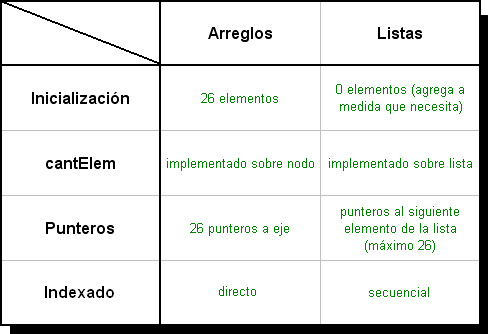
\includegraphics[scale=0.6]{./figuras/graficos/ej3/cuadrito.png} 
\label{fig:cuadrito}
\end{figure}

Como se dice en el cuadro comparativo, uno de los motivos es la inicializaci'on: el nodo sobre arreglo tendr'a consumido ya 26 elementos apenas se lo inicializa mientras que el nodo sobre lista comenzar'a vac'io y agregar'a hijos a medida que sea necesario. En cuanto a la contabilizaci'on de la cantidad de hijos, el nodo sobre arreglo debe contar con cantElem para poder saber cuantos hijos tiene tal nodo (as'i no tendremos que recorrer el arreglo cada vez que necesitemos saberlo), mientras que el nodo sobre listas no lo tiene, pero viene impl'icito con la lista, pues suponemos que la lista tiene dentro un mecanismo similar para evitar un recorrido innecesario. Hasta aqu'i podr'ia pensarse que la lista ocupar'a m'as lugar que los arreglos, pues cada nodo de la lista debe mantener un puntero al siguiente, pero no es as'i, pues el arreglo tambi'en tiene punteros, y los tiene en cada elemento, pues estamos comparando una lista de ejes con un arreglo punteros a eje.

El espacio utilizado lo medimos con una librer'ia que contiene cuatro headers: heap.h, heapfactory.h, memorymgr.h, memorypool.h. Esta librer'ia se encuentra adjunta en el cd. Simplemente agregando \textit{HeapFactory::GetDefaultHeap()->getPeak();} en una l'inea del c'odigo podremos obtener la mayor cantidad de memoria (en bytes) utilizada por el programa hasta el momento (el pico de memoria), o sea todo bloque de memoria que haya sido pedido por el c'odigo. Esto lo utilizamos haciendo una lista de palabras a agregar, y cada vez que agregamos una palabra, pedimos el pico.

\subsection{Resultados}

\subsubsection{Experiencia 1: Cantidad de operaciones al agregar palabras de largo creciente}
\begin{figure}[H]
\centering
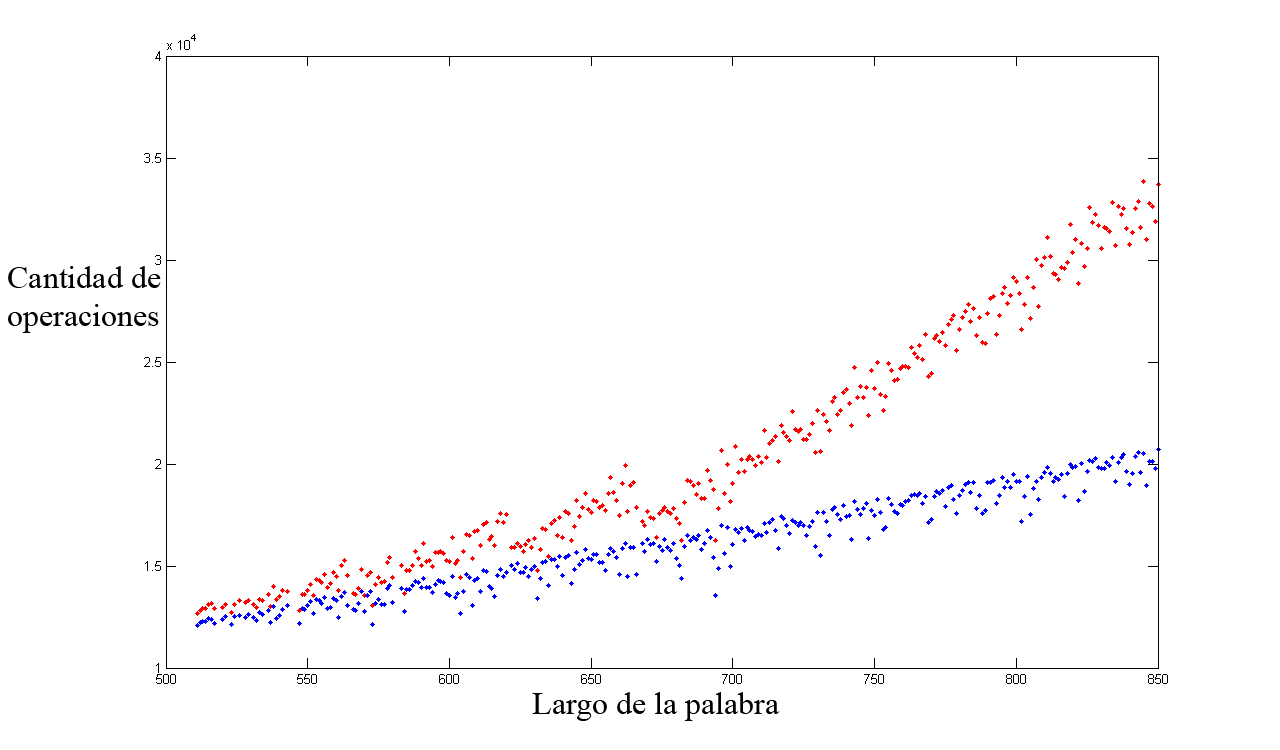
\includegraphics[scale=0.5]{./figuras/graficos/ej3/operacionesAgregar.png} 
\label{fig:ej3exp1}
\end{figure}
Los puntos rojos, corresponden a la implementaci'on con listas, los azules con arreglos.

\subsubsection{Experiencia 2: Cantidad de operaciones al buscar palabras de largo creciente}
\begin{figure}[H]
\centering
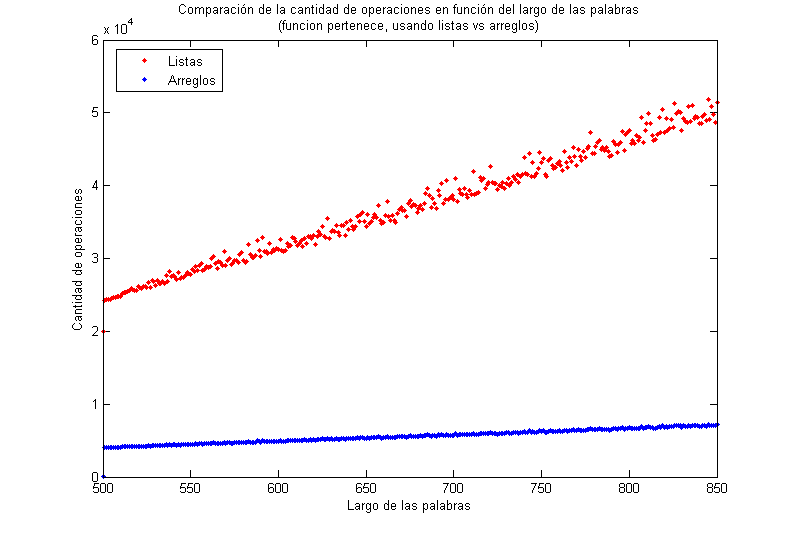
\includegraphics[scale=0.7]{./figuras/graficos/ej3/operacionesPertenece.png} 
\label{fig:ej3exp2}
\end{figure}

\subsubsection{Experiencia 3: Cantidad de operaciones al quitar palabras de largo creciente}
\begin{figure}[H]
\centering
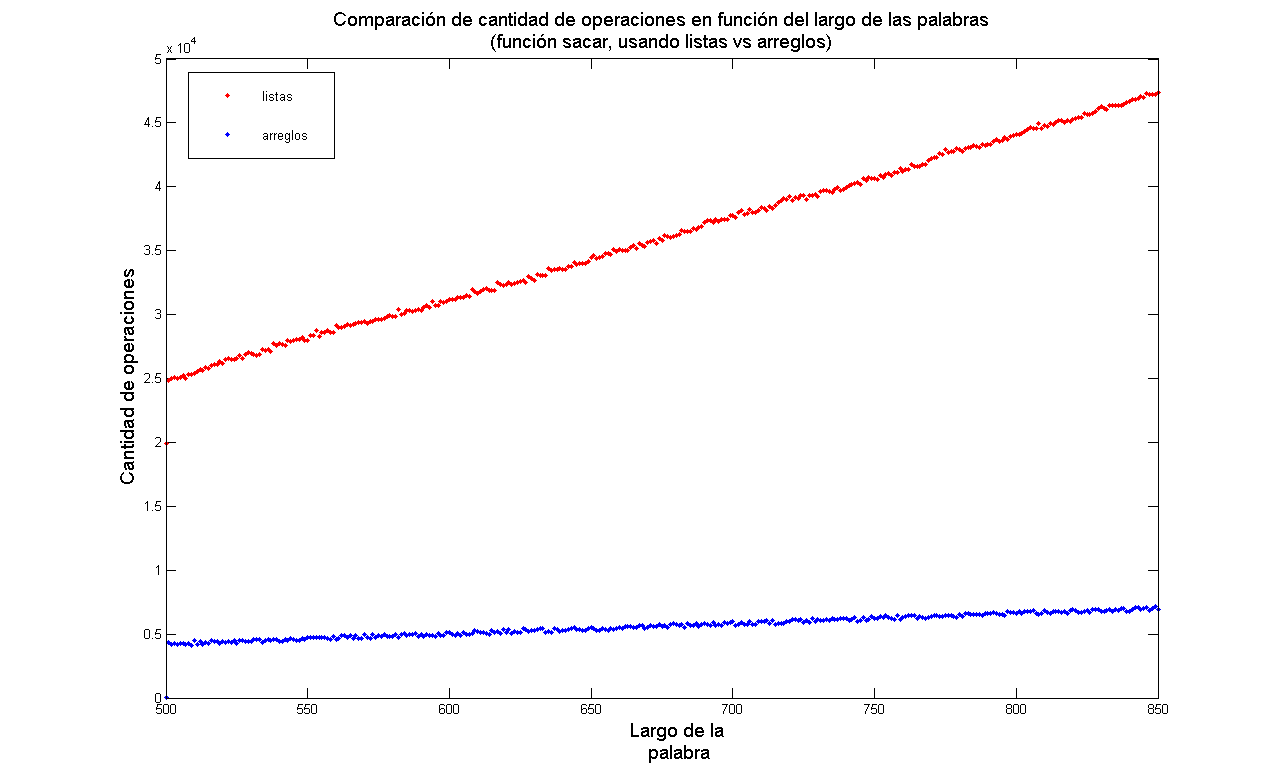
\includegraphics[scale=0.5]{./figuras/graficos/ej3/operacionesSacar.png} 
\label{fig:ej3exp3}
\end{figure}

%\subsubsection{Experiencia 4: Cantidad de operaciones al agregar palabras menores que alguna ya agregada}
%\begin{figure}[H]
%\centering
%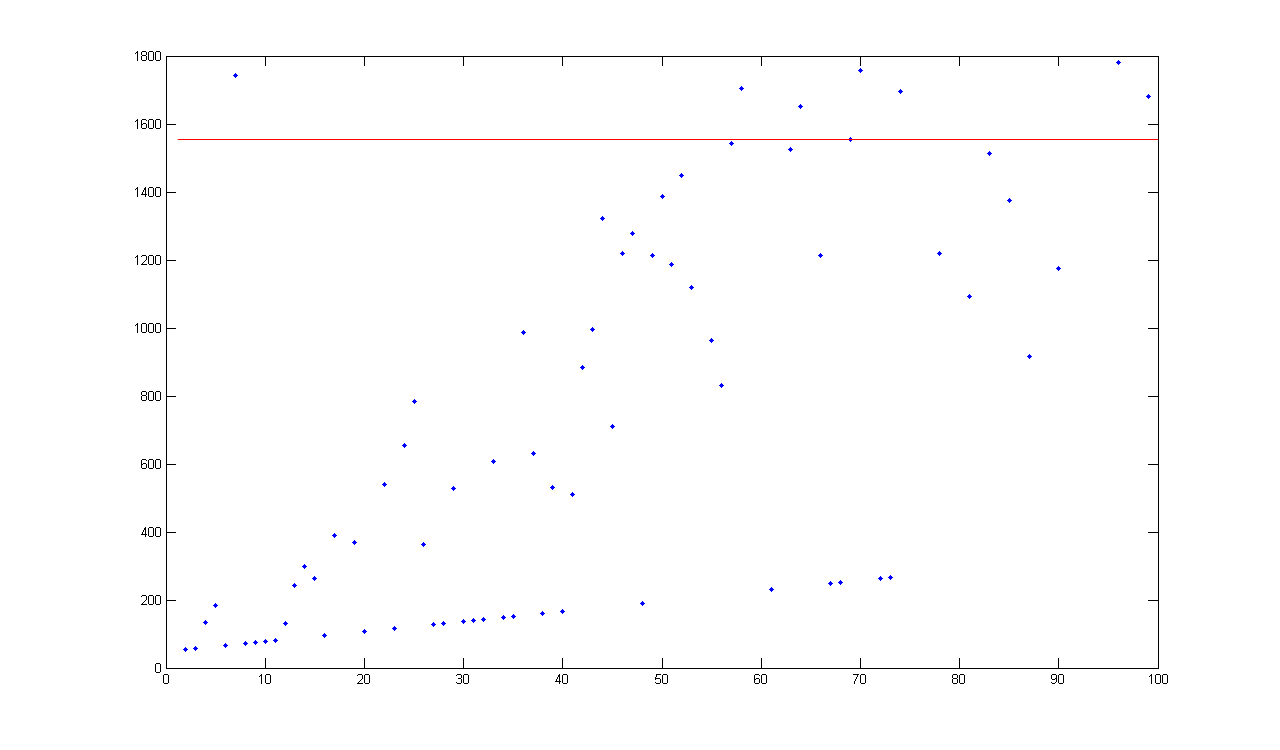
\includegraphics[scale=0.5]{./figuras/graficos/ej3/primeroMax.png} 
%\label{fig:ej3exp4}
%\end{figure}
%La linea roja indica la cantidad de operaciones de la cadena mas larga.

\subsubsection{Experiencia 5: Tiempo requerido para agregar diferentes conjuntos de palabras}
\begin{figure}[H]
\centering
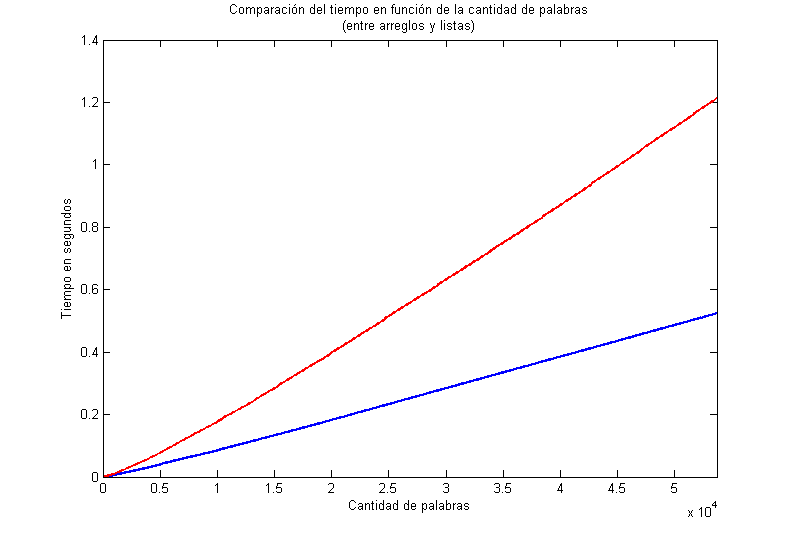
\includegraphics[scale=0.7]{./figuras/graficos/ej3/comparacionArreglosListas.png} 
\label{fig:ej3exp4}
\end{figure}
En rojo con listas, azul con arreglos.

\subsubsection{Experiencia 6: Cantidad de memoria utilizada para diferentes conjuntos de palabras de caso promedio}
\begin{figure}[H]
\centering
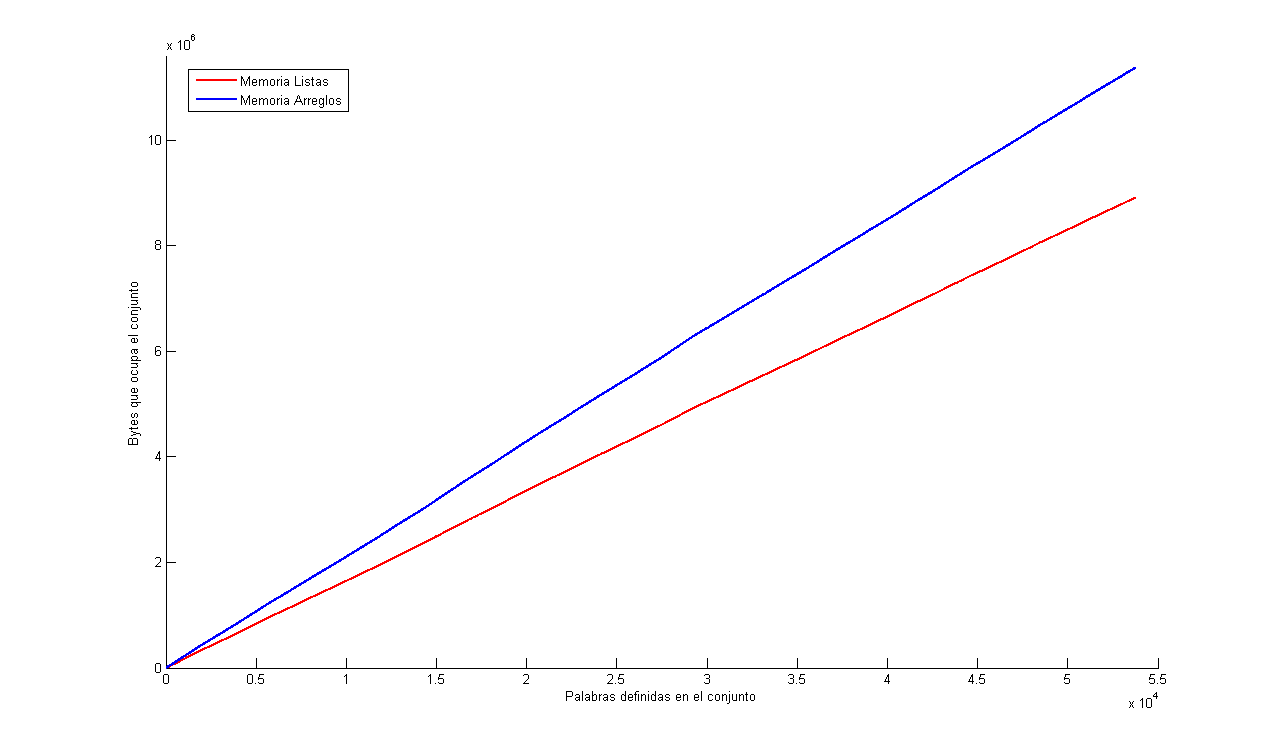
\includegraphics[scale=0.5]{./figuras/graficos/ej3/memoria.png} 
\label{fig:ej3exp5}
\end{figure}

\subsubsection{Experiencia 6: Cantidad de memoria utilizada para diferentes conjuntos de palabras de peor caso}
\begin{figure}[H]
\centering
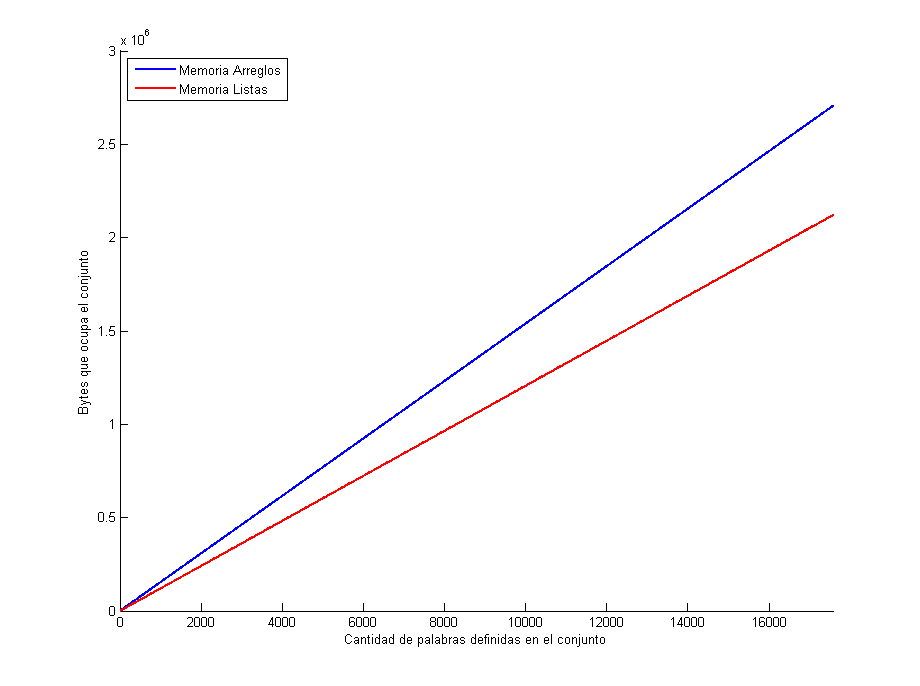
\includegraphics[scale=0.5]{./figuras/graficos/ej3/memoriaPeorCaso.png} 
\label{fig:ej3exp5}
\end{figure}

\subsection{Discusi�n}
En las experiencias 1, 2 y 3 observamos como la cantidad de operaciones es considerablemente mayor en la implementaci'on con listas, esto es de esperarse ya que encontrar el eje por el cual bajar es mucho m'as r'apido en los arreglos, si bien en ambos es O(1), las listas presentan una constante mucho mas alta, ya que si un nodo tiene 26 hijos la b'usqueda es lineal y se recorren en peor caso los 26 ejes.

Independientemente de la implementaci'on se noto como la cantidad de operaciones se incrementa linealmente a medida que se agregan palabras m'as largas, esto es de esperarse ya que la complejidad nos dio O($long_{max}$).

%FIXME: esto me parece que vuela porq no sabemos si esta bien fundamentado
%En la figura 4, lo que vemos es que en general la cantidad de operaciones es menor que la cantidad de operaciones del m'aximo, no obstante hay algunos casos donde se obtiene un n'umero de operaciones mayor. Esto creemos que no se contradice con lo que esperabamos, sino que lo podemos explicar considerando que si bien la primer palabra es la mas larga, agregarla es facil, ya que no hay otros nodos, entonces el costo principal esta en copiar la cadena, en cambio en otros casos, hay que copiar la cadena, partir nodos y recorrer ejes, por esta raz�n puede dar mas operaciones que el caso m'aximo.

La experiencia 5 vuelve a poner de minifiesto lo que observamos anteriormente, es decir que la implementaci'on con arreglos es m'as veloz que la implementaci'on con listas.

Finalmente la experiencia 6 nos muestra como la implementaci'on con arreglos, que se mostr'o claramente m'as r'apida, consume una gran cantidad de memoria m'as que la implementaci'on con listas para todo caso. Esto confirma nuestra previa comparacion entre ambas implementaciones, y es una buena raz'on por la cual podr'ia considerarse, pese a que es m'as lenta, la implementaci'on sobre listas antes que sobre arreglos.

A modo de conclusi'on podemos decir en primer lugar que el las experiencias coincidieron con lo calculado te'oricamente. Y por otro lado observamos como cada implementaci'on de los nodos presenta sus ventajas y desventajas, raz'on por la cual para utilizar una u otra implementaci'on debe considerarse el contexto donde se va a usar, es decir, a la hora de utilizar una u otra, es importante plantearse que es mas cr'itico: si el tiempo de respuesta (nodos con arreglos) o la utilizaci'on de la memoria (nodos con listas).
